\documentclass[]{article}  % Comment this line out

%\IEEEoverridecommandlockouts                              % This command is only
                                                          % needed if you want to
                                                          % use the \thanks command
%\overrideIEEEmargins

\usepackage[margin=1in]{geometry}
\usepackage{amsmath}    % need for subequations
\usepackage{graphicx}   % need for figures
\usepackage[font=footnotesize,labelfont=footnotesize]{caption}
\usepackage{verbatim}   % useful for program listings
\usepackage{color}      % use if color is used in text
%\usepackage{begin{subfigure} % use for side-by-side figures
\usepackage{subcaption}
\usepackage{hyperref} % use for hypertext links, including those to external documents and URLs
\usepackage{multirow}
\usepackage{rotating}
\usepackage{array}
\usepackage{xspace}
\usepackage{indentfirst}
\usepackage{amssymb}
\usepackage{float}
\usepackage{algorithm}
\usepackage{algpseudocode}
\usepackage{comment}
\usepackage{sidecap}
\usepackage{booktabs}

\newtheorem{theorem}{\bf Theorem}
\newtheorem{todo}{\bf Todo}
\newtheorem{remark}{\bf Remark}
\newtheorem{corollary}{\bf Corollary}
\newtheorem{definition}{\bf Definition}
\newtheorem{lemma}{\bf Lemma}
\newtheorem{proposition}[theorem]{\bf Proposition}

\title{Iterating the Polygon Visibility Decomp Algorithm}

\author{Alexandra Q. Nilles% <-this % stops a space
%\thanks{This work was partially supported by National Science Foundation (award numbers CMMI-1100579 and IIS-1302393).}
}

\begin{document}

This algorithm proceeds by shooting rays from each vertex to all the visible
reflex vertices. If the resulting ray lands inside an open segment of $\delta
P$, the intersection point is added to a vertex set $v\_new$, which is then
inserted into $\delta P$ when all the ray shooting operations have completed.

Each reflex vertex induces a combinatorial change in the
visibility polygon for points on either side of the resulting new vertex. This
is because the originating vertex, from the original polygon, is visible on one
side of the ray but not the other.

In pseudocode, the algorithm proceeds as

\begin{algorithm}
\caption{Partition the boundary of a polygon into visibility
equivalence classes.}
\label{algo:insert}
\begin{algorithmic}
\Procedure{PartitionPoly}{$poly$}
\State $reflex\_verts \gets$ \Call{GetReflexVerts}{$poly$}
\For{$v_r$ in $reflex\_verts$}
    \For{$v_{vis}$ in \Call{VisibleVerts}{$poly, v_r$}} \Comment{vertices
visible from reflex induce transitions}
        \State $v_{new} \gets$ \Call{ShootRay}{$v_{vis}, v_r$}
    \EndFor
\EndFor
\State $P_{ins} \gets$ \Call{InsertVerts}{$v_{new}, poly$}
\State \textbf{return} $P_{ins}$
\EndProcedure
\end{algorithmic}
\end{algorithm}

The resulting polygon, with $v\_new$ inserted, has the following property:

\begin{quotation}

The visibility polygons of any two points in the same open segment have the same
combinatorial structure with respect to the original polygon $P$. The edge-edge
visibility graph is the same for both visibility polygons, and there is a
continuous transformation from one visibility polygon to another, without
adding or deleting edges.

\end{quotation}

One notable condition of this property is that it holds only with respect to the
original polygon $P$, not the new polygon $P_{ins}$.

But since we are using the edge-edge visibility properties of $P_{ins}$ to do
navigation, it might be nice to have this visibility-invariance property to hold
for visible edges in $P_{ins}$.

Perhaps we can just iterate the original algorithm until convergence, at which
point all segments will be guaranteed to have this property with respect to
$P_{ins}$.

This appears to be possible for some polygons:

\begin{figure}
\centering
\begin{subfigure}{0.6\textwidth}
  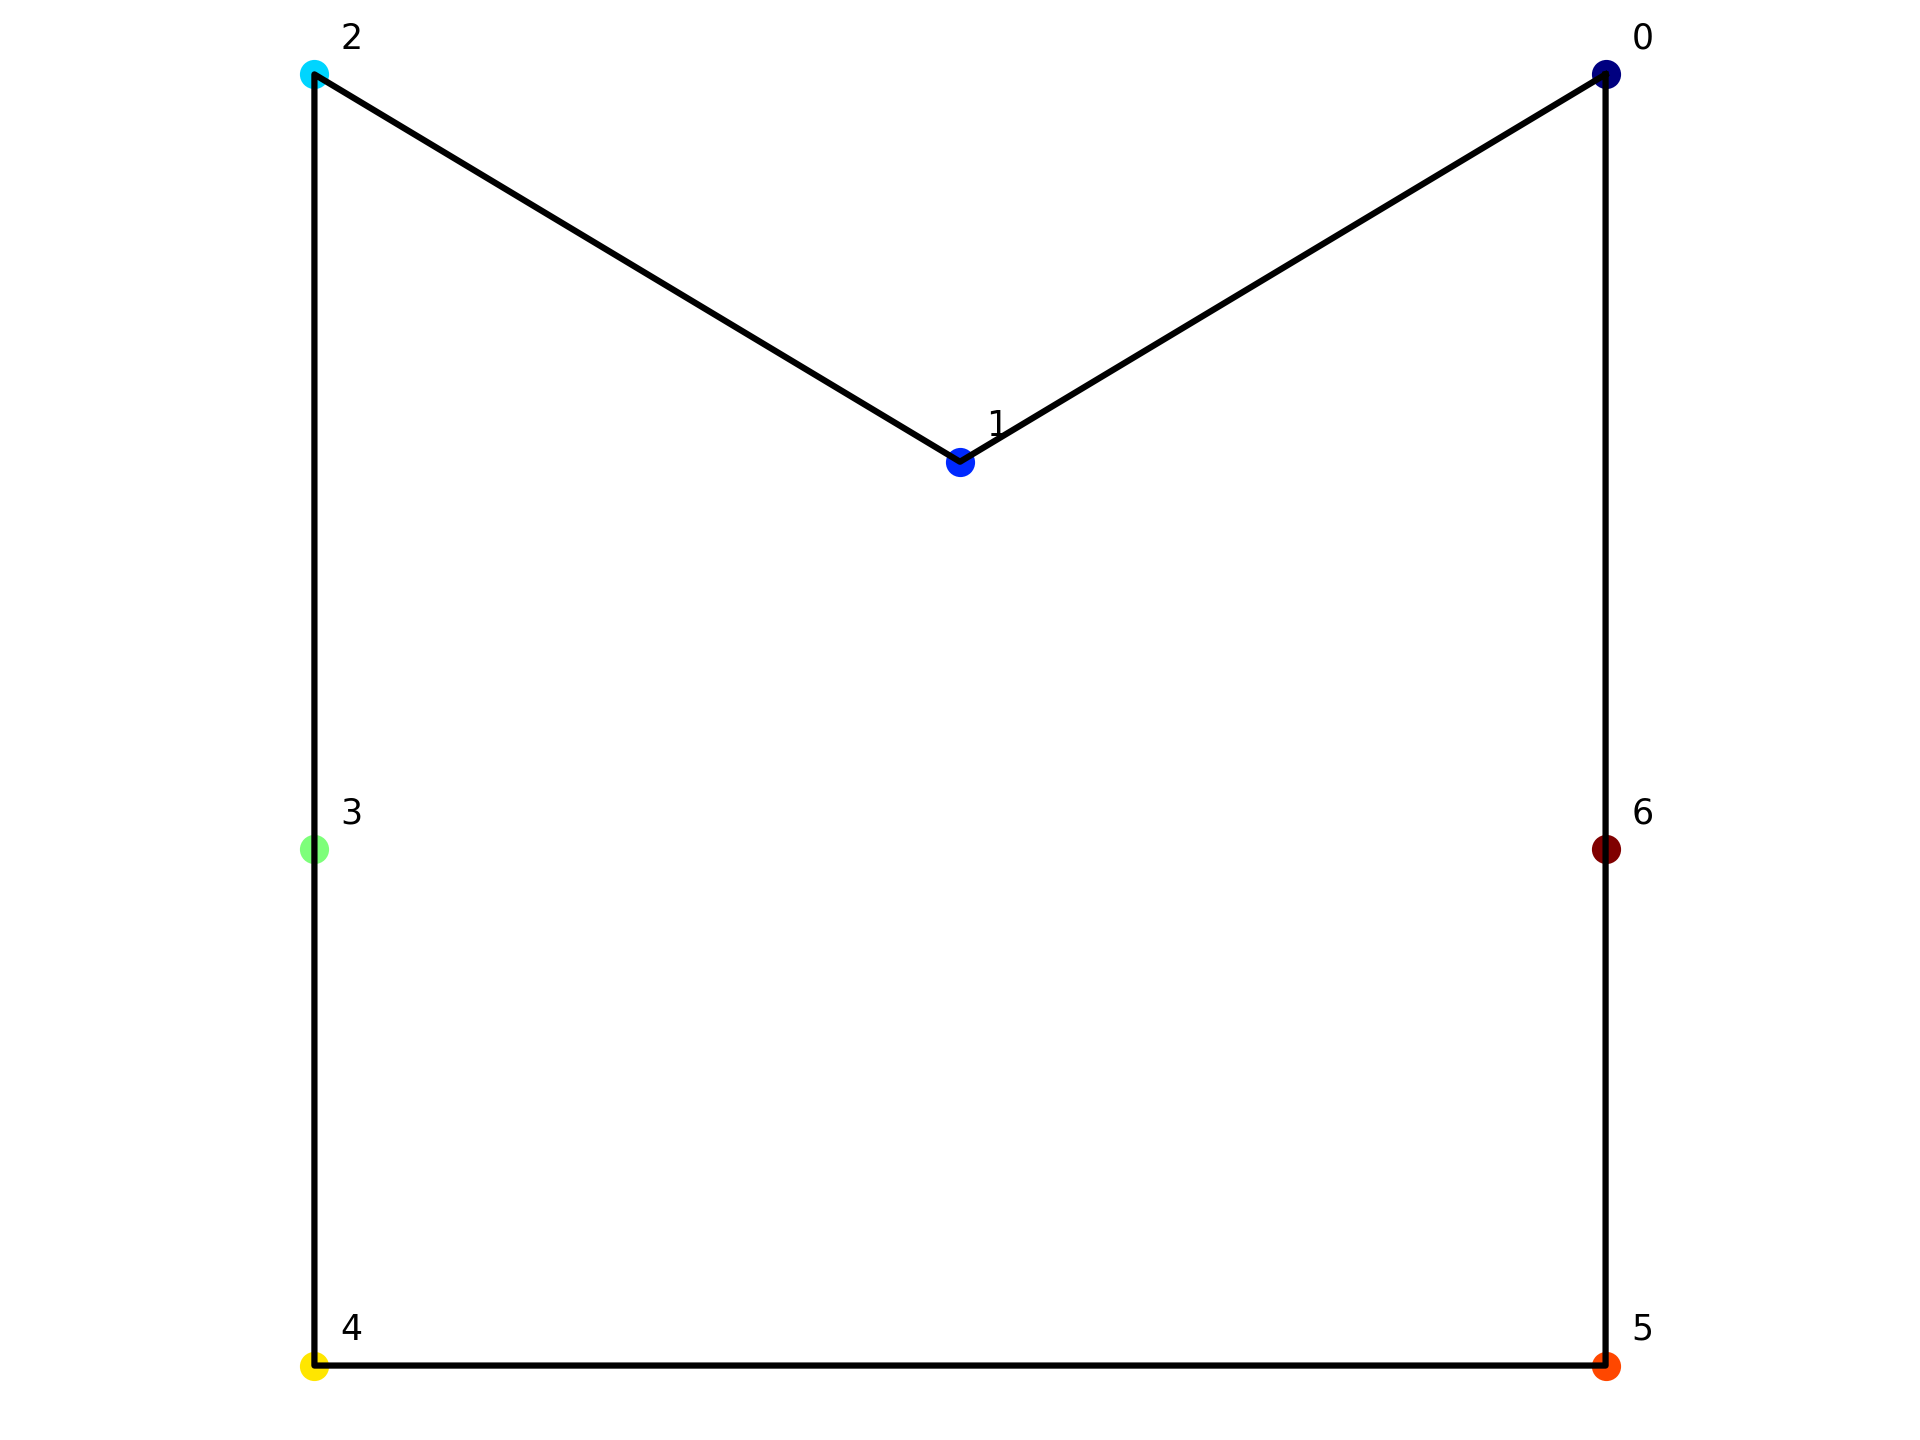
\includegraphics[width=\textwidth]{figures/iter1.png}
\end{subfigure}

\begin{subfigure}{0.6\textwidth}
  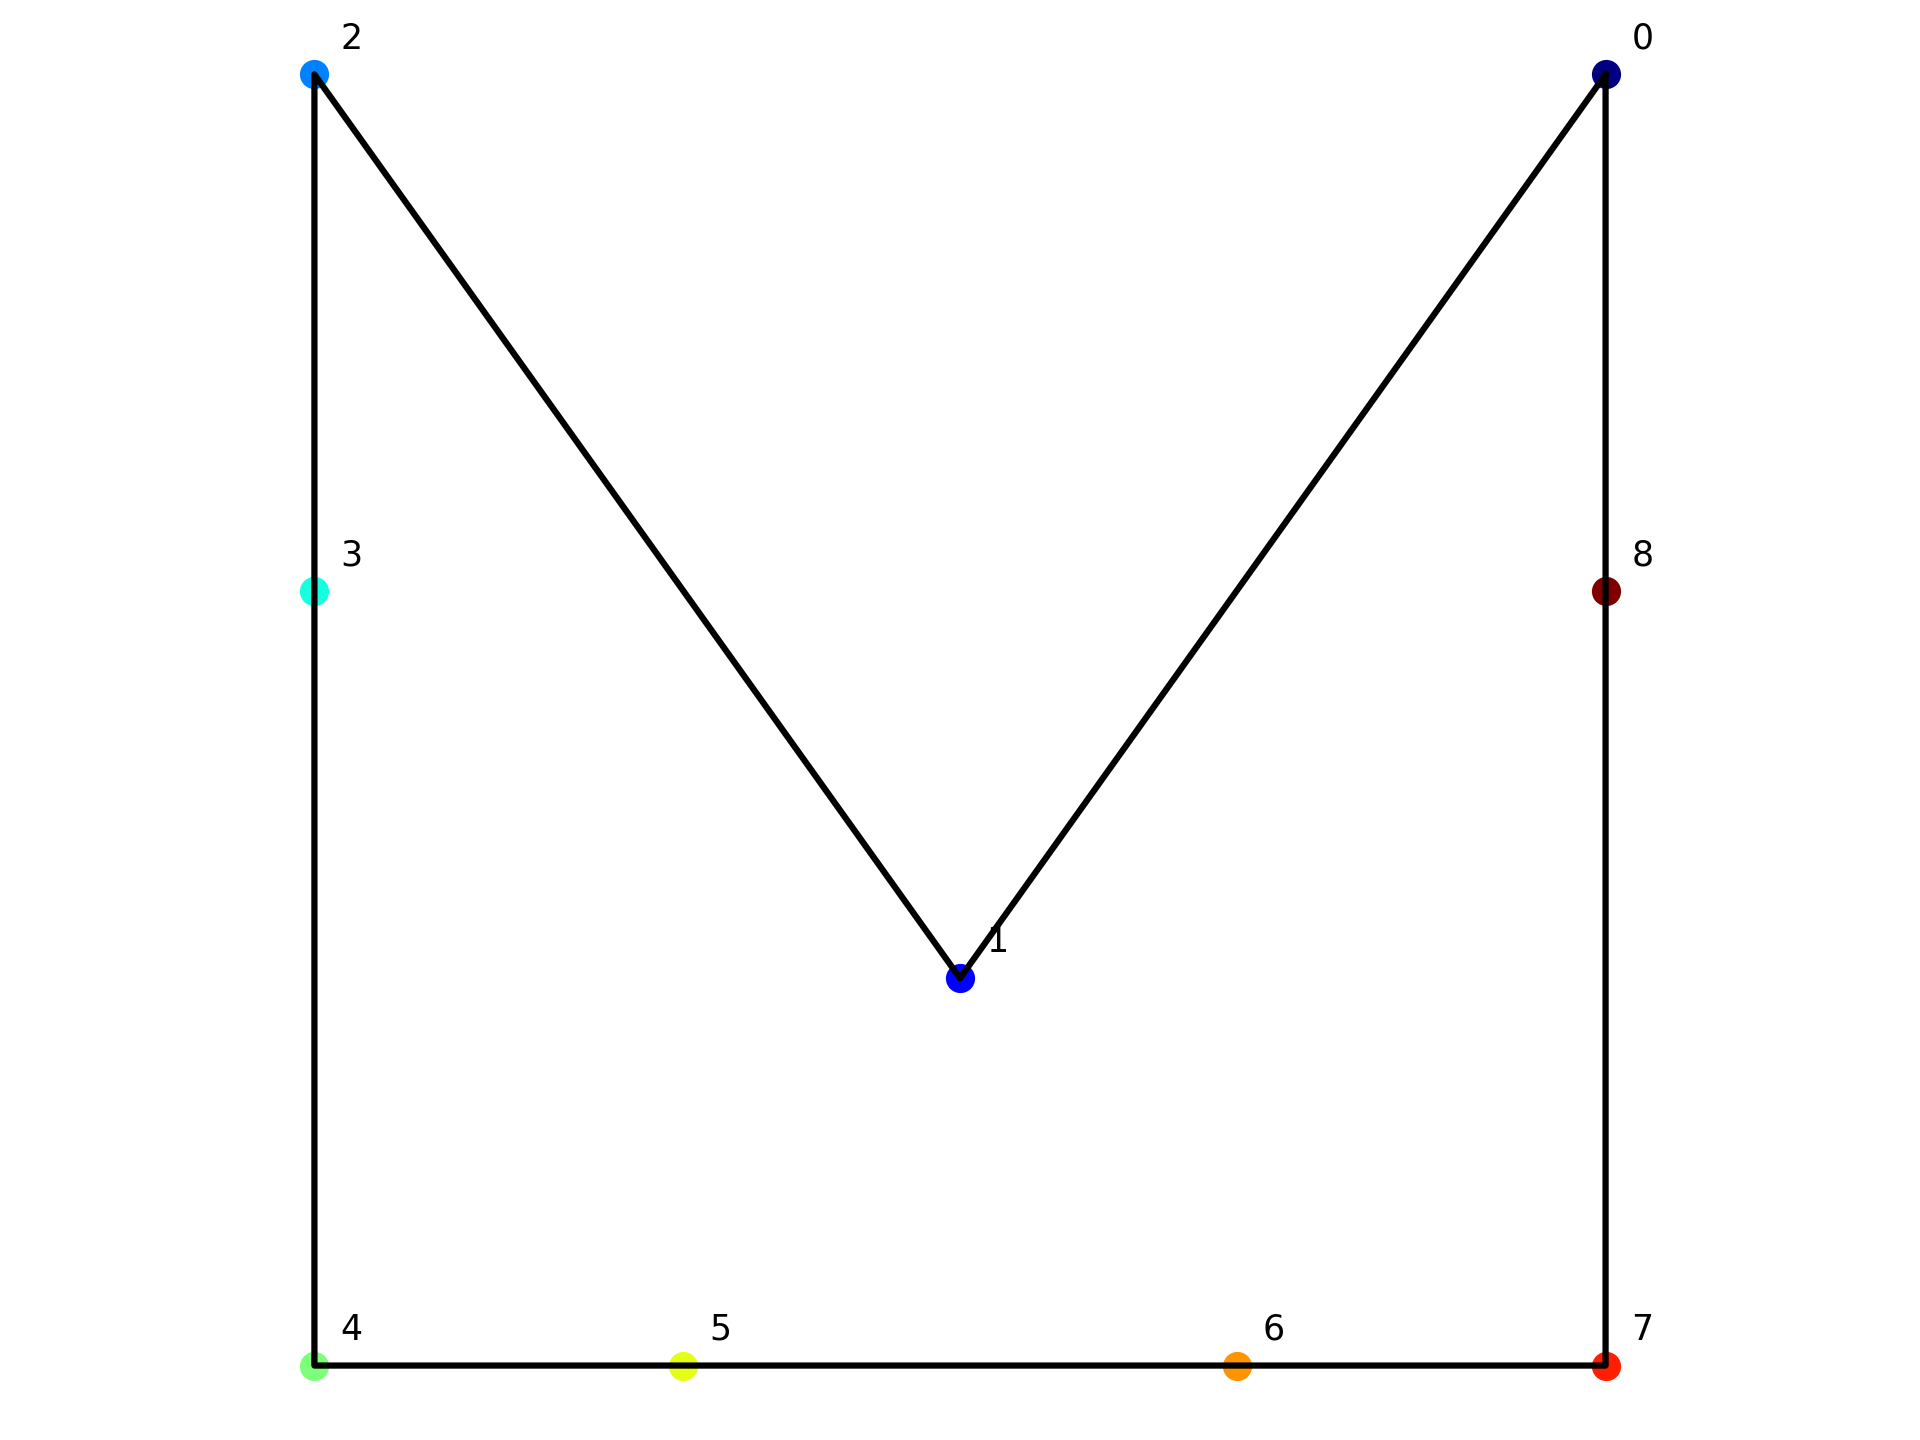
\includegraphics[width=\linewidth]{figures/iter2.png}
\end{subfigure}

\begin{subfigure}{0.6\textwidth}
  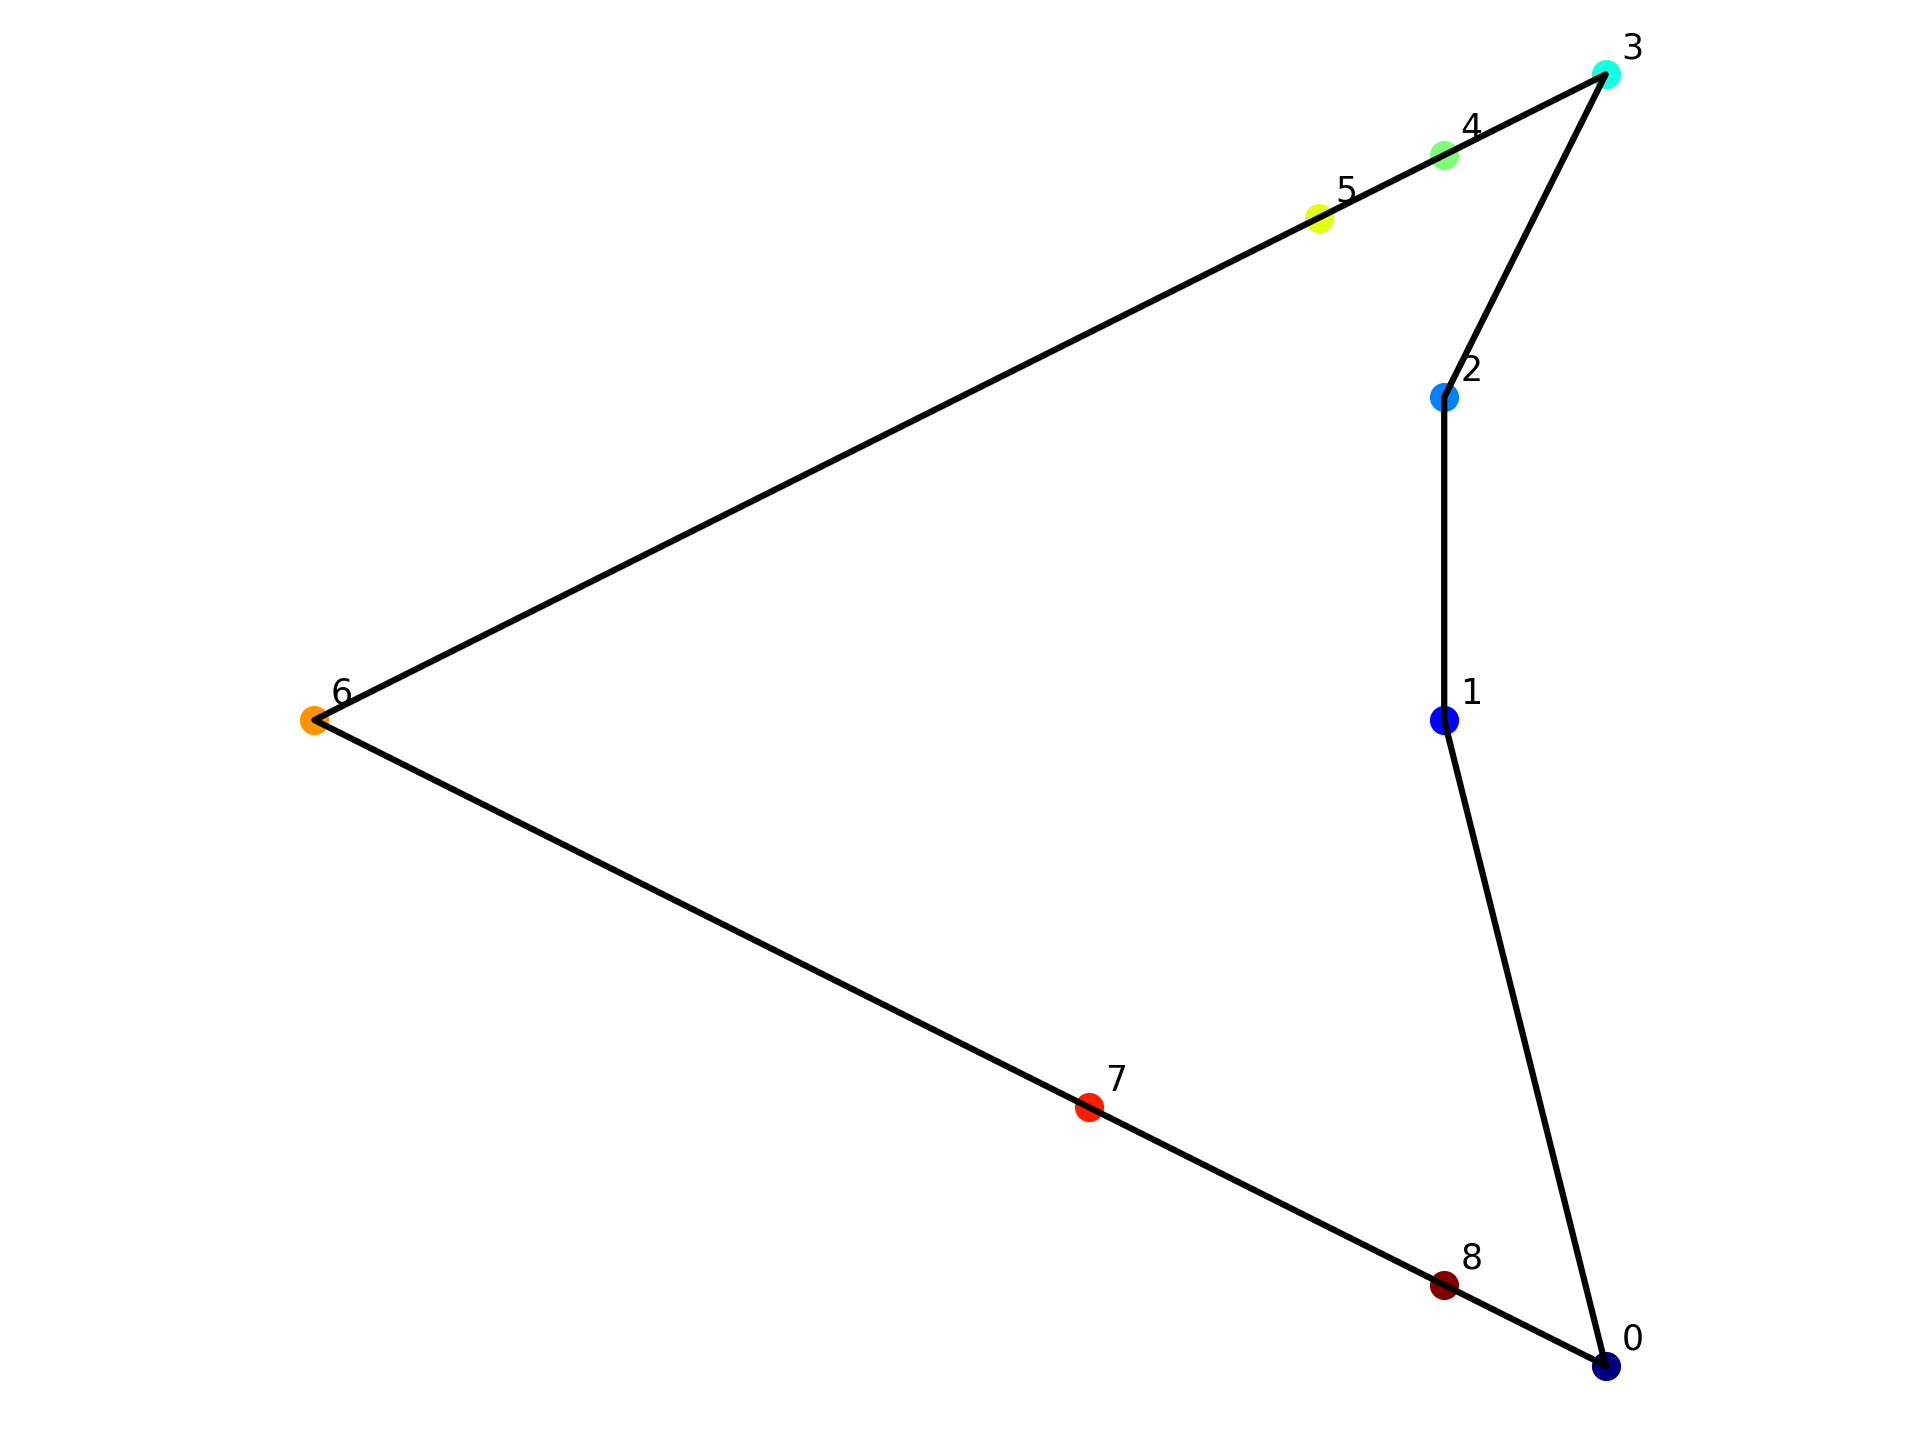
\includegraphics[width=\linewidth]{figures/iter3.png}
\end{subfigure}
\caption{Polygons where the decomposition algorithm terminates in one
iteration.}
\end{figure}

\newpage

But other polygons do not seem to converge. We can keep iterating this
example, and each iteration adds two more vertices (one for each reflex). 
At some point it hits the limits of machine precision and appears to
converge. Interestingly, it appears to converge toward the line tangent to both
reflex vertices (the bitangent).

\begin{figure}
\centering
\begin{subfigure}{0.6\textwidth}
  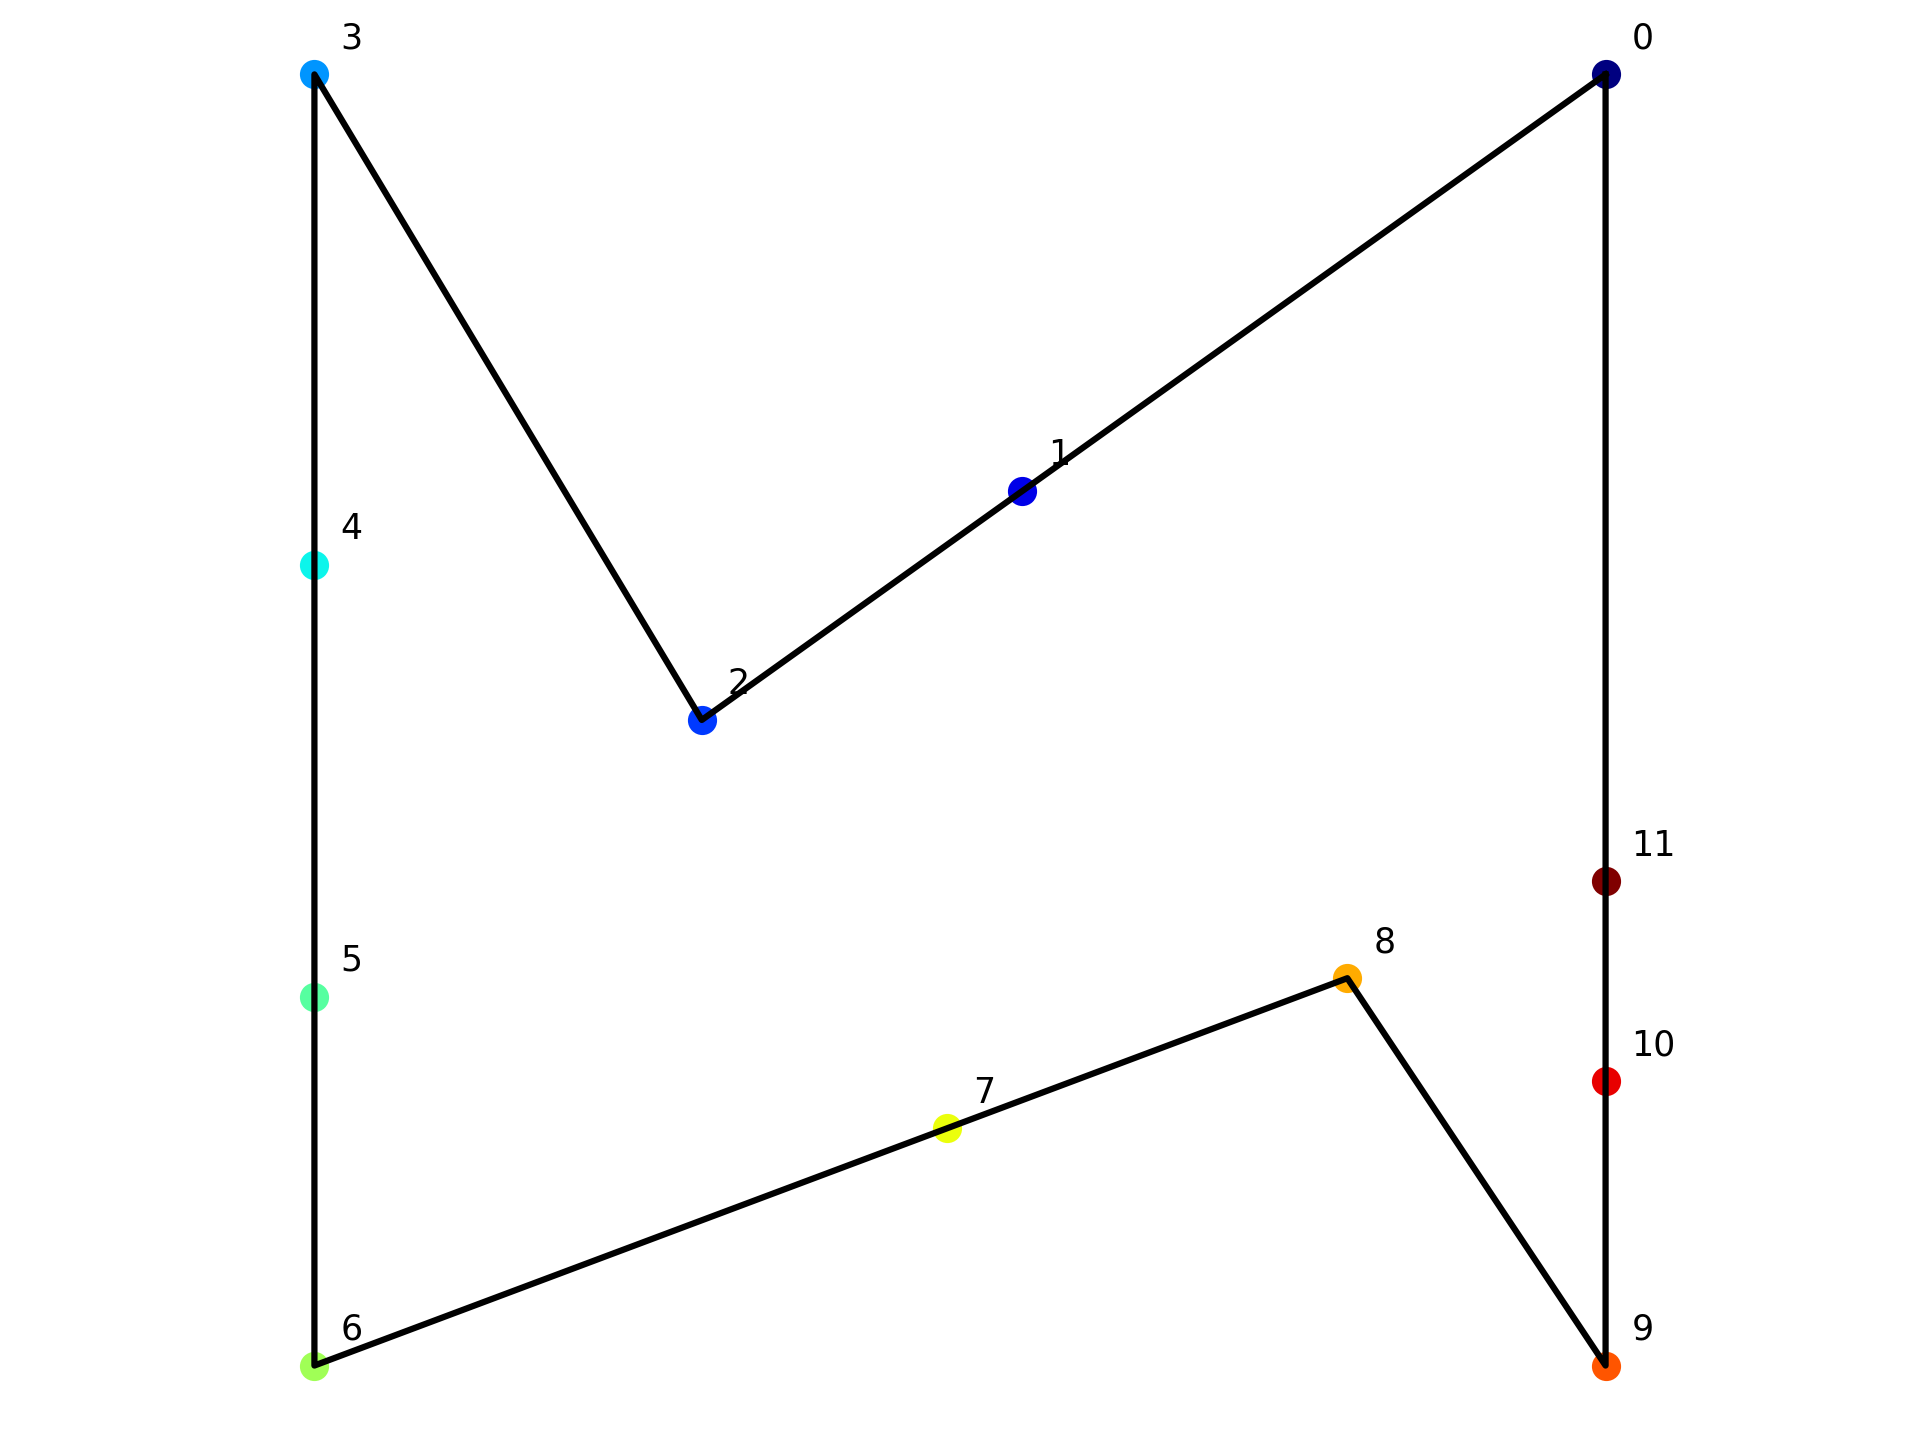
\includegraphics[width=\textwidth]{figures/iterbit1.png}
\end{subfigure}

\begin{subfigure}{0.6\textwidth}
  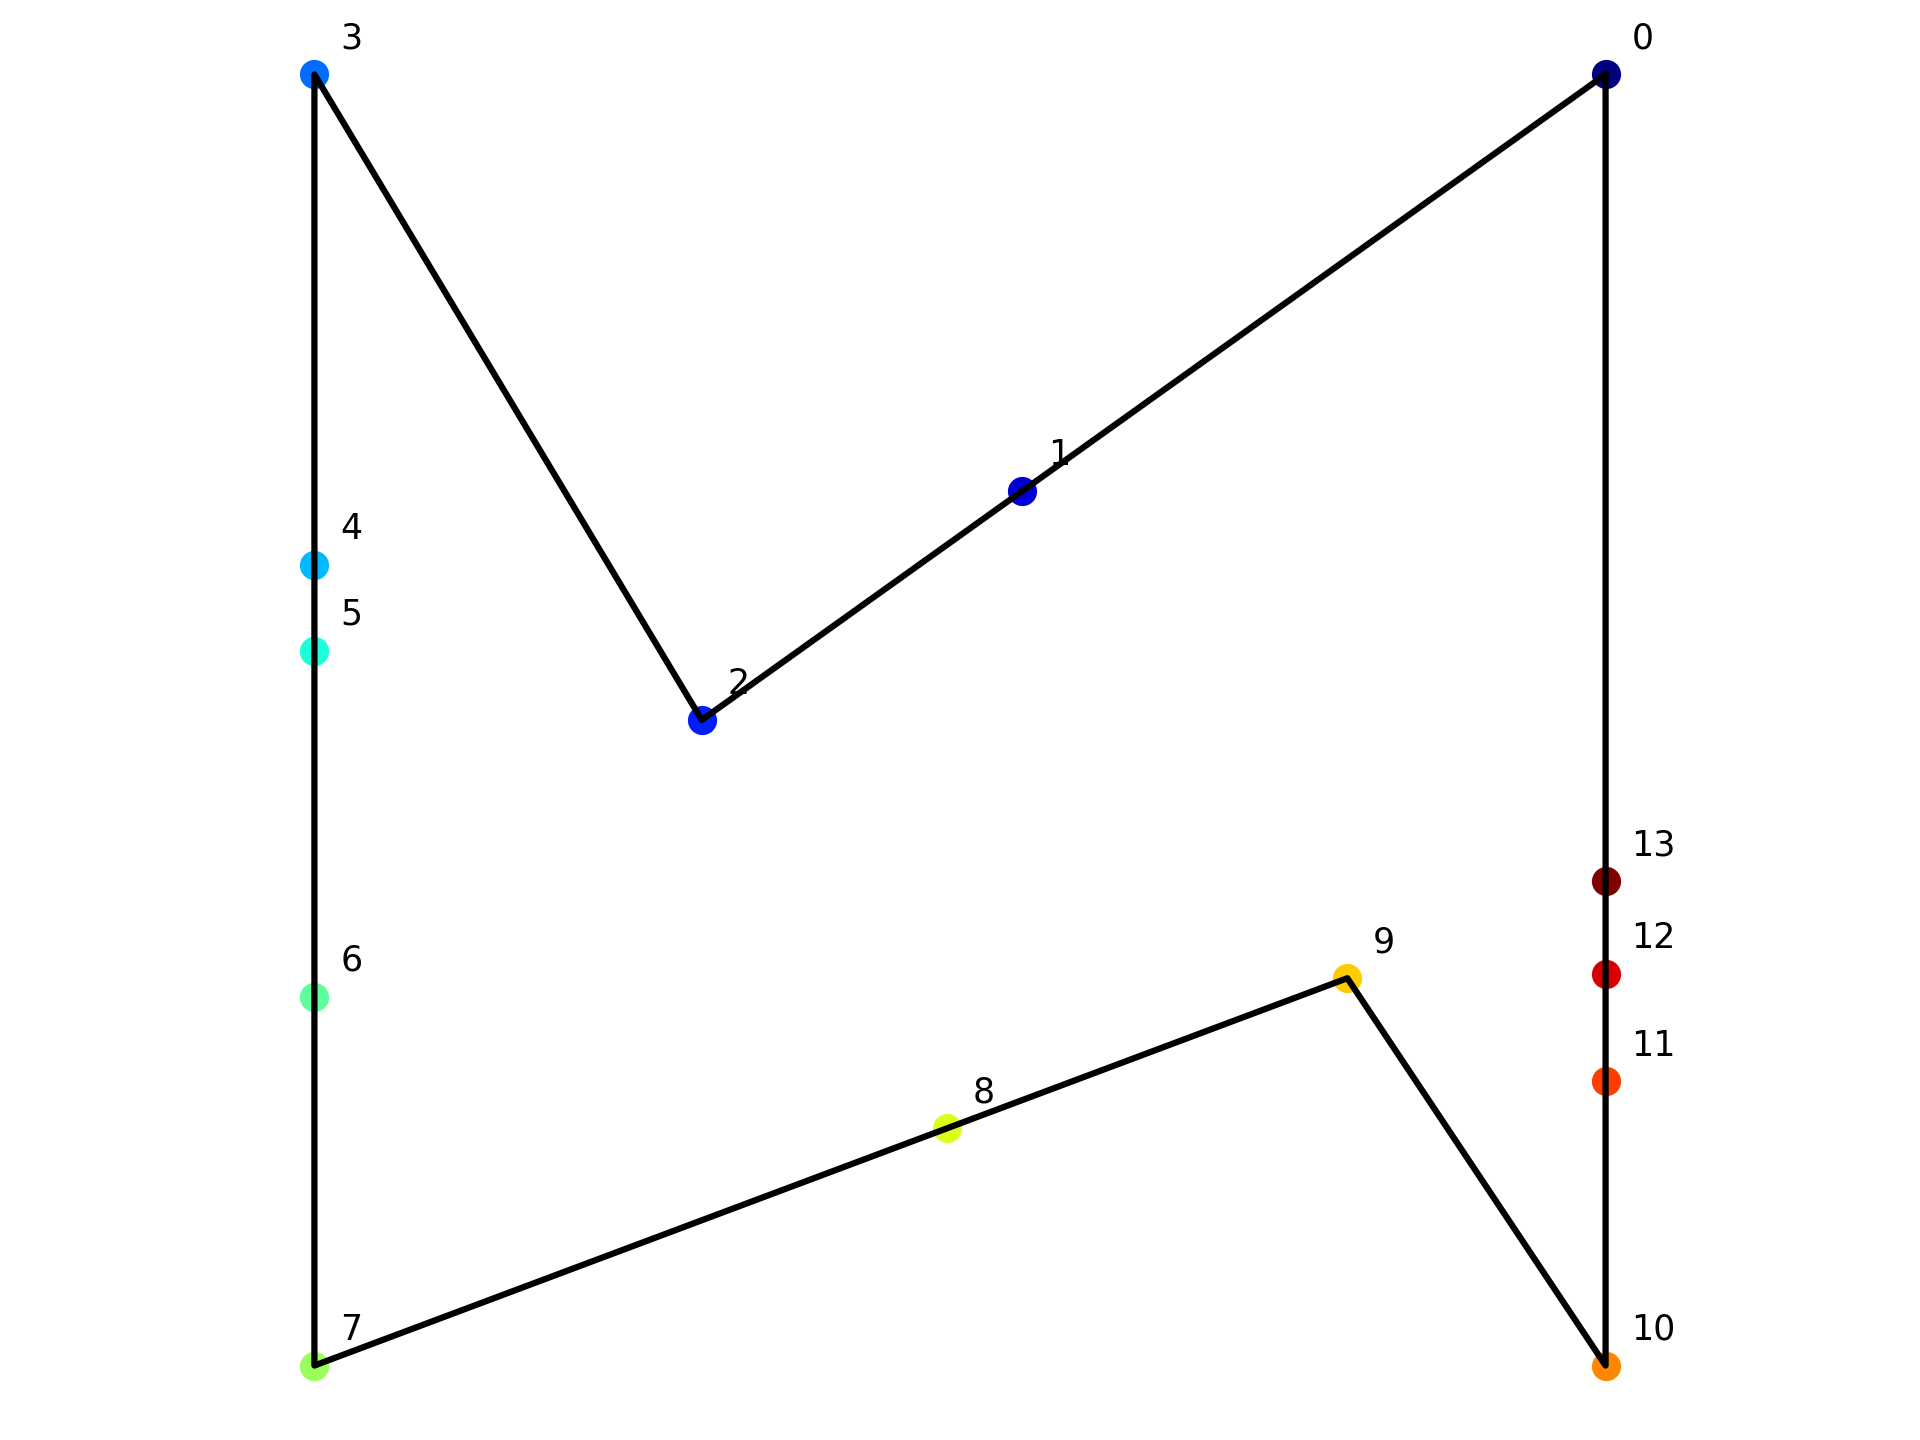
\includegraphics[width=\linewidth]{figures/iterbit2.png}
\end{subfigure}

\begin{subfigure}{0.6\textwidth}
  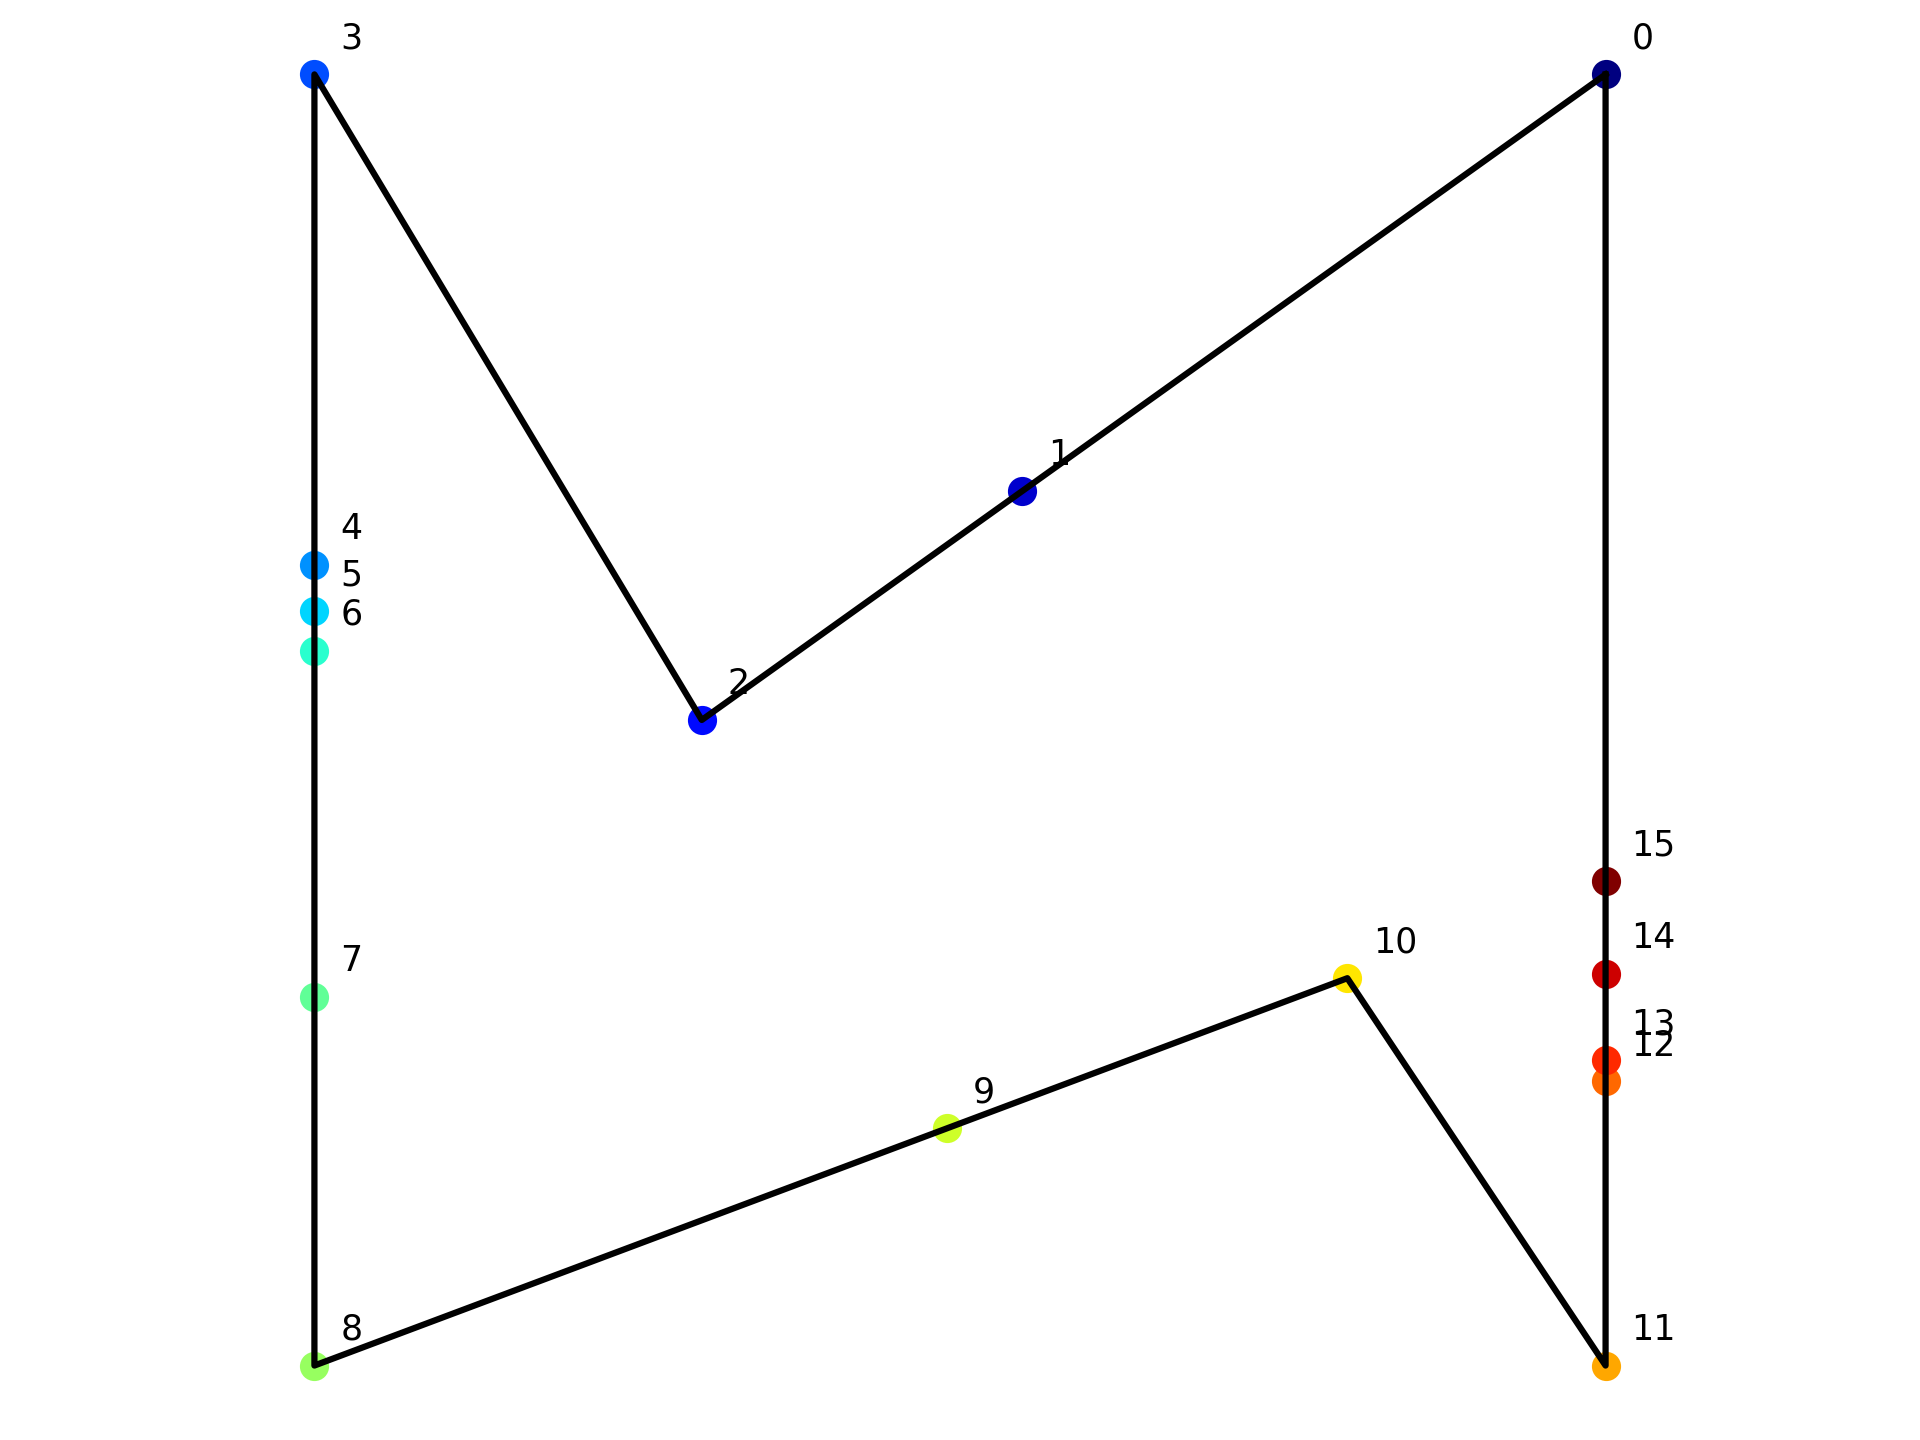
\includegraphics[width=\linewidth]{figures/iterbit3.png}
\end{subfigure}
\caption{}
\end{figure}


\end{document}
